\section{Introduction}

Over the past few decades, there has been a significant shift in computing and storage from PC-like clients to smaller, often mobile devices coupled with expansive internet services. 
Simultaneously, traditional enterprises are increasingly adopting cloud computing. This shift offers numerous benefits, including ease of management and ubiquitous access for users.

For vendors, Software-as-a-Service (SaaS) accelerates application development and facilitates easier implementation of changes and improvements. 
Software fixes and enhancements are streamlined within data centers, eliminating the need for updates across millions of clients with diverse hardware and software configurations. 
Hardware deployment is simplified to a few well-tested configurations.

Server-side computing allows for the rapid introduction of new hardware devices, such as hardware accelerators or platforms, and supports many application services at a low cost per user. 
Certain workloads require substantial computing power, making data centers a more natural fit compared to client-side computing.

\subsection{Geographical distribution of data centers}
Frequently, multiple data centers serve as replicas of the same service to reduce user latency and enhance serving throughput. 
Requests are typically processed entirely within one data center.
\begin{definition}[\textit{Geographic area}]
    Geographic areas partition the world into sectors, each defined by geopolitical boundaries.
\end{definition}
Within each geographic area, there are at least two computing regions. 
Customers perceive regions as a more detailed breakdown of the infrastructure. 
Notably, multiple data centers within the same region are not externally visible. 
The perimeter of each computing region is defined by latency (with a round trip latency of two milliseconds), which is too far for synchronous replication but sufficient for disaster recovery.
\begin{definition}[\textit{Availability zone}]
    Availability zones represent more granular locations within a single computing region.
\end{definition}
Availability zones enable customers to operate mission-critical applications with high availability and fault tolerance to data center failures by providing fault-isolated locations with redundant power, cooling, and networking. 
Application-level synchronous replication among availability zones is implemented, with a minimum of three zones being adequate for ensuring quorum.
\begin{figure}[H]
    \centering
    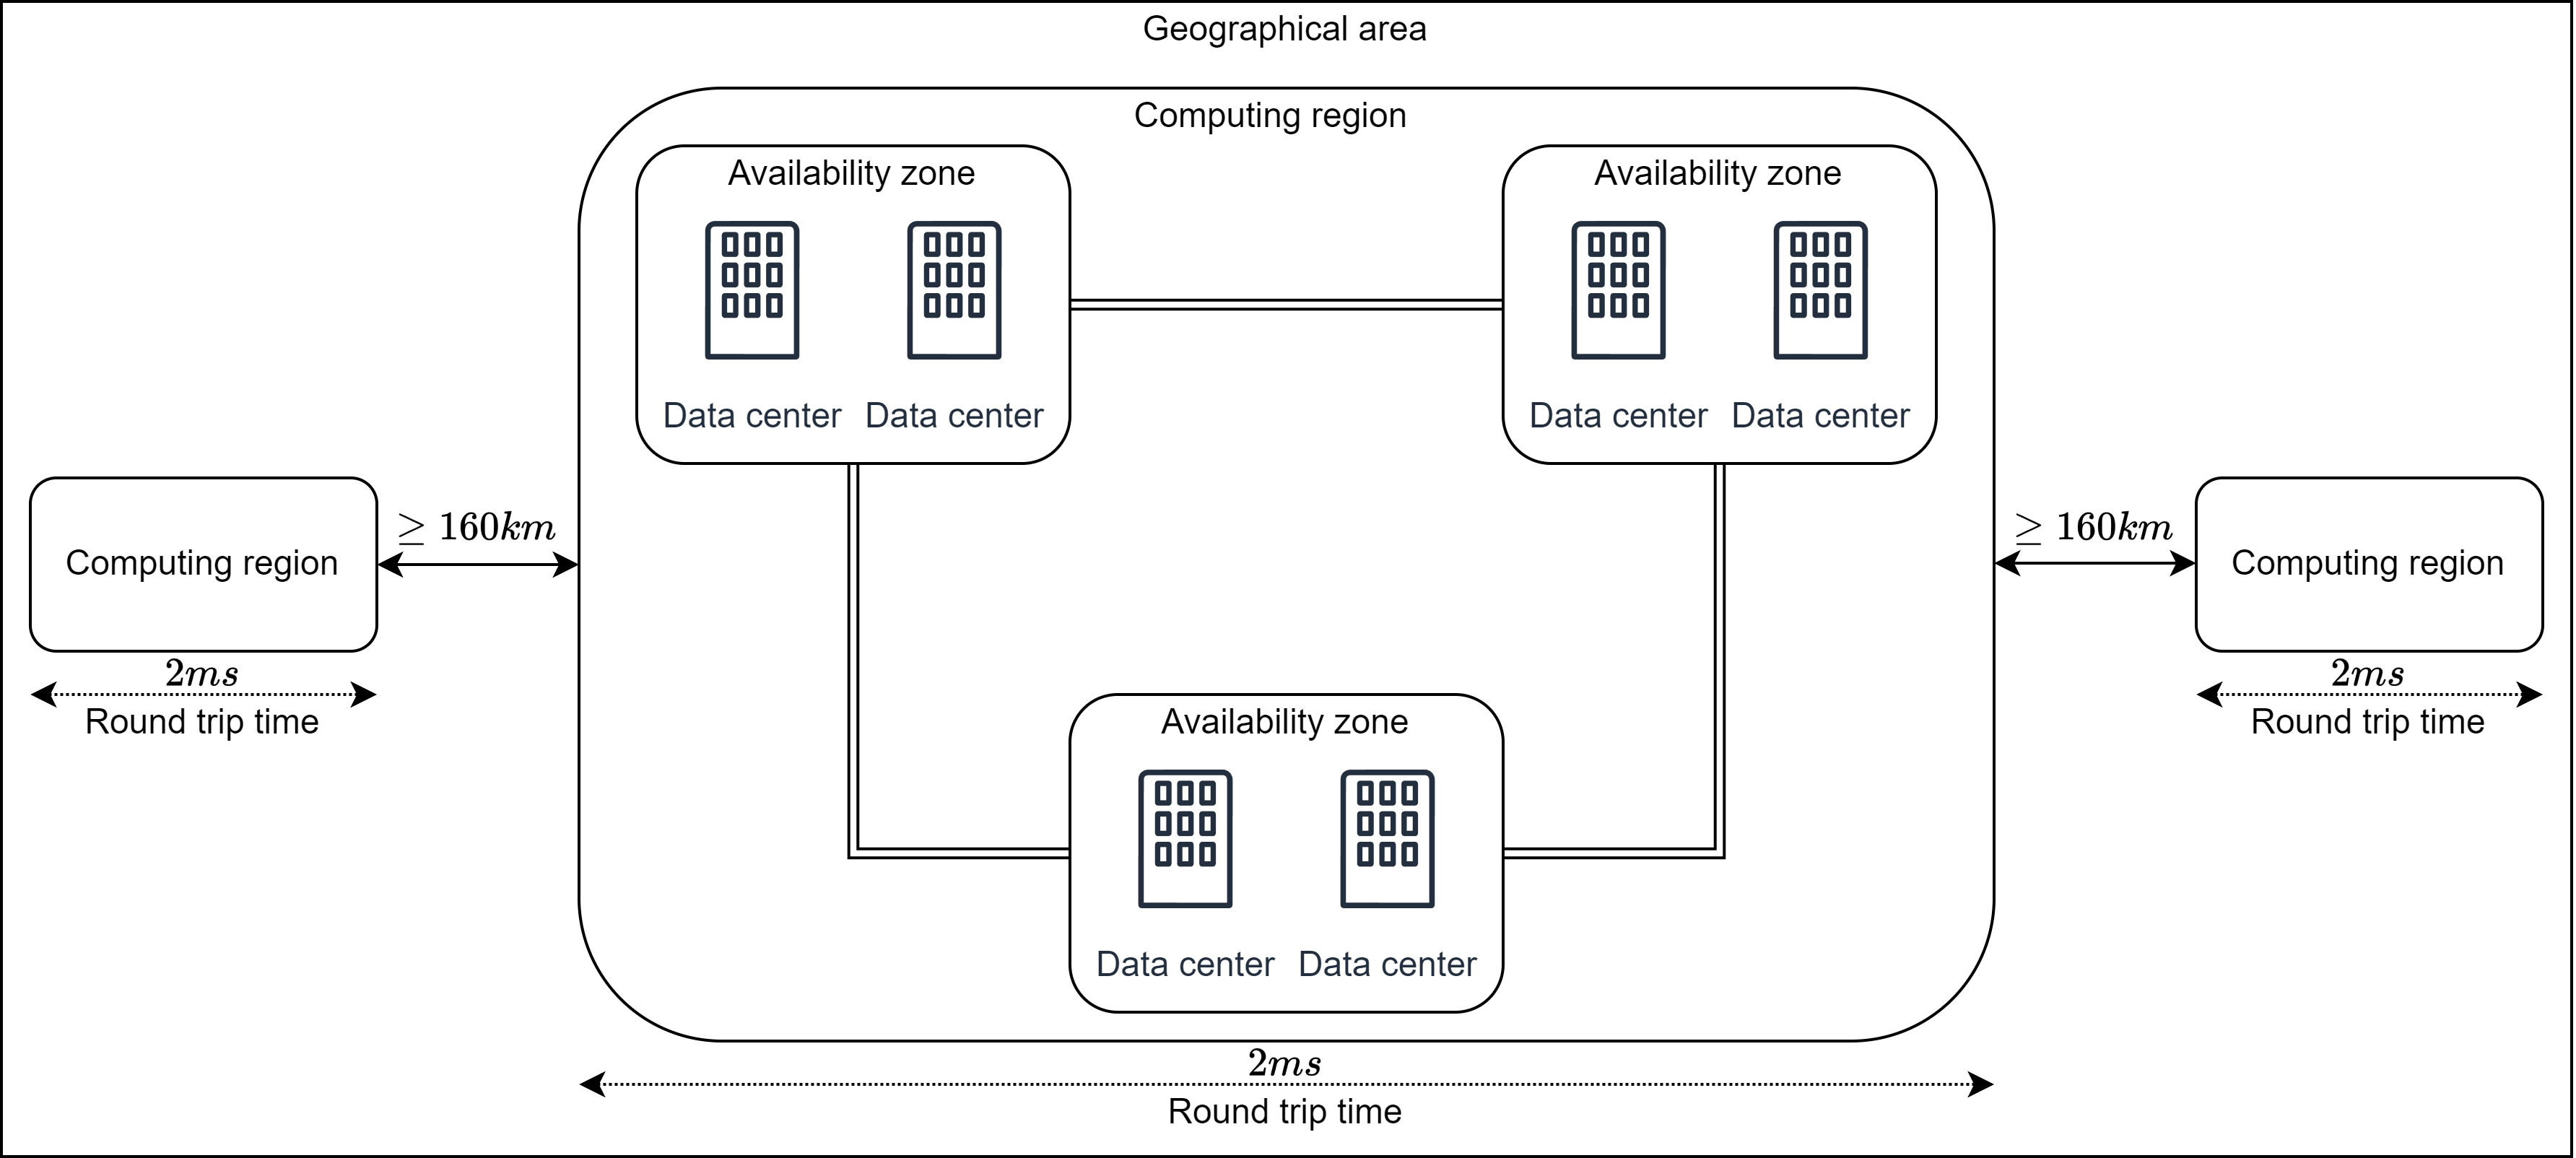
\includegraphics[width=1\linewidth]{images/computing.png}
    \caption{Geographical area structure}
\end{figure}